\documentclass[a4paper,11pt,oneside,openany]{jsbook}
%
\usepackage{fancyhdr}
\usepackage{amsmath,amssymb}
\usepackage{bm}
\usepackage[dvipdfmx]{graphicx}
\usepackage{subfigure}
\usepackage{url}
\usepackage{verbatim}
\usepackage{wrapfig}
\usepackage{ascmac}
\usepackage{fancyvrb}
\usepackage{makeidx}
\usepackage{comment}
\usepackage{float}

%%%%%%%%%%ここより上は必要なスタイルを読み込みたい時にのみ編集%%%%%%%%%%%%%
\usepackage{myjlab}
\makeindex
%%%%%%%%%% 念のため \usepackegeの一番下に myjlab があるように%%%%%%%%%%%%%

%%%%%%%%%%基本情報設定変更の必要なし%%%%%%%%%%%%%%%%%%%%%%%%%%%%
\def\daigaku{青山学院大学}
\def\gakubu{社会情報学部}
\def\gakka{社会情報学科}
\def\syubetsu{卒業論文}
\def\labname{宮治研究室}
\def\chiefexaminer{宮治 裕 准教授}

%%%%%%%%%%%%%%%%%%%%%%%%%%%%%%%%%%%%%%%
% ここから先「ここまで個人設定」の範囲に
% 各自の固有の情報を記入して下さい
%%%%%%%%%%%%%%%%%%%%%%%%%%%%%%%%%%%%%%%
\def\nendo{2013年度}
\def\teisyutsu{2014年~~1月}

\def\snum{15387019}
\def\jname{宮治 裕}
\def\thesistitle{宮治研における論文作成について} %タイトルを記入
\def\thesissubtitle{\LaTeX の利用} %サブタイトルを記入 ない場合はコメントアウトし,titlepage.tex を読み込むように変更


%%%%%%%%%% ここまで個人設定 %%%%%%%%%%%%%%


% 以下3行編集不要
\begin{document}
\linesparpage{30} %行数指定
\mojiparline{35} %文字数指定


%%%%%%%%%%%%%%%%%%%%%%%%%%%%%%%%%%%%%%%
% ここから先「ここまでタイトル表示設定」の範囲は
% サブタイトル有りの場合とサブタイトルなしの場合の
% 条件に応じてコメントアウト部分を変更して下さい
%%%%%%%%%%%%%%%%%%%%%%%%%%%%%%%%%%%%%%%
\begin{titlepage}
\begin{center}{\large
\nendo ~~\daigaku ~\gakubu ~~\syubetsu
}
\end{center}
\begin{flushright}

{\large
指導教員: \chiefexaminer \\ % 主査
%副査:□□□□ 教授              % 副査
}
\end{flushright}
\begin{center}
\vspace*{150truept}
{\huge \thesistitle}\\ % タイトル
\vspace{10truept}
{\Large ―~\thesissubtitle~―}\\ % サブタイトル(なければコメントアウト)
\vspace{150truept}
%\vspace{120truept}
{\Large
\begin{tabular}{rl}
%{\Large 学籍番号 \snum}\\ % 学籍番号
学籍番号 & \hspace{1zw}{\snum}\\
%{\Large \jname}\\ % 著者
 & \\
氏名 & \hspace{1zw}{\jname}\\
\end{tabular}
}\\
\vspace{70truept}
{\large \teisyutsu}\\ % 提出日
\end{center}
\end{titlepage}
%サブタイトル有りの場合
%\begin{titlepage}
\begin{center}{\large
\nendo ~~\daigaku ~\gakubu ~~\syubetsu
}
\end{center}
\begin{flushright}

{\large
指導教員: \chiefexaminer \\ % 主査
}
\end{flushright}

\begin{center}
\vspace*{150truept}
{\huge \thesistitle}\\ % タイトル
\vspace{170truept}
%\vspace{120truept}
{\Large
\begin{tabular}{rl}
%{\Large 学籍番号 \snum}\\ % 学籍番号
学籍番号 & \hspace{1zw}{\snum}\\
%{\Large \jname}\\ % 著者
 & \\
氏名 & \hspace{1zw}{\jname}\\
\end{tabular}
}\\
\vspace{70truept}
{\large \teisyutsu}\\ % 提出日
\end{center}
\end{titlepage}%サブタイトル無しの場合

%%%%%%% ここまでタイトル表示設定 %%%%%%%%%%


% ------------------- ここから先「ここまで共通」の範囲は編集不要 --------------------
\frontmatter
%%% 論文要旨
\chapter*{論文要旨}
%\thispagestyle{empty}
\addcontentsline{toc}{chapter}{論文要旨}

近年,大学進学という選択肢は高校生にとって一般的な選択肢として受け入れられるようになった.
また2020年4月から高等教育の修学支援制度が施行される予定であり,この制度の施行により大学進学率は増加すると考えられる.
さらに新設大学,新設学部も年々増加しているなかで,特定の大学に志願者が集中するという問題が提起されている.

本研究では,高校生が自分にあった適切な大学を選択できるように支援するシステムを考案した.
ネットの大学に関する記事から大学ごとの単語ベクトルを生成し,大学間の類似度を測る.
また,キャンパスの所在地や学部ごとの偏差値といったデータを利用して,大学間の潜在的な関係性の可視化を支援するシステムを構築した.

検証の結果,特定の大学に絞ったシステムを構築し,潜在的な関係性の可視化を実現した.
また,より横断的なデータを利用したシステムの精度向上の可能性に関して示した.

% abstract.texの中は \chapterなど書かずに単なるテキストを入力する

%%% 謝辞
\chapter*{謝辞}
%\thispagestyle{empty}
\addcontentsline{toc}{chapter}{謝辞}
本研究を進めるにあたって,親身にご指導していただいた指導教官の宮治教授に厚く御礼申し上げます.
並びに,多くの助言,ご指摘いただいた研究室の先輩方と後輩の皆様に感謝の意を表します.

また学習に使用したデータとして大学プレスセンターの記事を利用させていただいた,株式会社大学通信の皆様,パスナビのデータを利用させていただいた旺文社の皆様に感謝の気持ちと御礼を申し上げます.
最後に家庭内で体調面,精神面で支えて下さった父と母に心から感謝を述べ,謝辞にかえさせていただきます.
% thanks.texの中は \chapterなど書かずに単なるテキストを入力する

%%% 目次
\tableofcontents
\mainmatter
% ------------------- ここまで共通 -------------------


%%%%%%%%%%%%%%%%%%%%%%%%%%%%%%%%%%%%%%%
% ここから先「ここまで論文本文」の範囲を
% 各自の章立てや付録にあわせて編集して下さい
%%%%%%%%%%%%%%%%%%%%%%%%%%%%%%%%%%%%%%%

%%% 本文ここから chap1 chap同様に必要なだけ章を入れる
\chapter{はじめに}
本論文では,大学に関する記事から文書毎のベクトルを生成することで各大学毎の特色をデータ化し,潜在的な関係性を可視化する研究について記述する.

まず,本研究をおこなう背景となった事柄について述べる.
次に,研究目的の詳細について述べ,最後に次章以降の本論文の構成について概略を述べる.

\section{背景}
近年,大学進学という選択肢は高校生にとって,一般的な選択肢として受け入れられるようになった.
図 \ref{fig:univ_continuance_rate}に過去10年間の大学・短大進学率と,大学(学部)進学率の推移を文部省公表\cite{univContinuanceRate}の資料から示す.  
直近3年間の推移は比較的横ばい傾向にあるが,高校卒業後の進路に関して50\%近い学生が大学へ進学している.

更に,2020年4月から高等教育の修学支援制度\cite{Shingakusyusienseido}が施行される.
この新制度では,学生個人に対する要件と,支援対象者の所得に関する要件を満たした場合に授業料などを減免するか,給付型の奨学金を支給する.
対象となる学校種は大学,短期大学,高等専門学校,専門学校となる.
この制度の施行により,大学・専門学校進学率は今後増加すると考えられる.  
\begin{figure}[H]
\centering
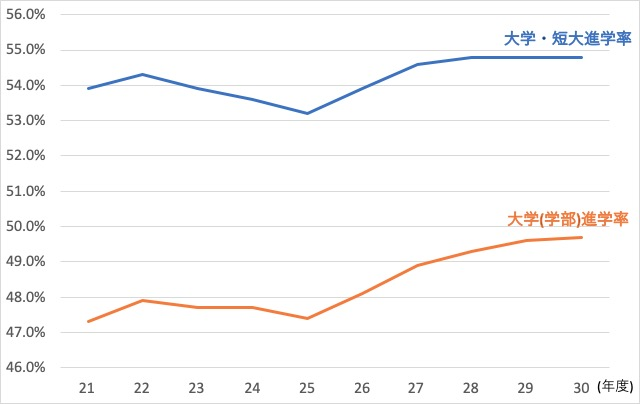
\includegraphics[height=8cm]{images/univ_continuance_rate.jpg}
\caption{過去10年間の大学進学率推移}
\label{fig:univ_continuance_rate}
\end{figure}

一方大学の学校数に関して,日本では774校存在している\ref{fig:university_num}.これは2019年4月の入学者を募集した大学の数である.
それぞれの内訳としては,国立大学が82大学,公立大学が91大学,私立大学が592大学であり,私立大学が全体の約8割を占めている.
このデータのうち,2019年度新設大学は13大学で,内訳は公立大学1校,私立大学10校,専門職大学2校に上る.
また新設学部は国立,私立専門職大学合わせて61学部,新設学科は計118学科となっている.

志願者数の観点から,大学に関する志願者数の推移を日本私立大学振興・共済事業団の資料\cite{shigan}からまとめた.
\begin{figure}[H]
\centering
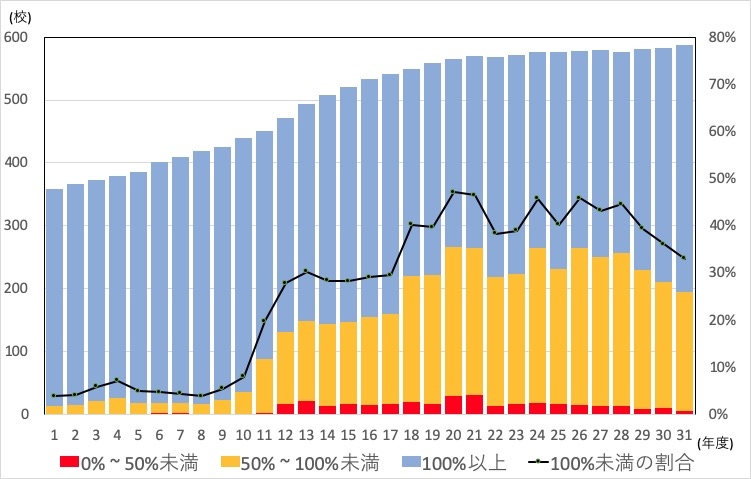
\includegraphics[height=8cm]{images/shigansya.jpg}
\caption{平成元年〜31年の私立大学志願者数の推移}
\label{fig:shigan}
\end{figure}
大学数は増加傾向にあったものの,ここ10年間はほぼ横ばいである.
志願者数が募集人数を下回った大学の比率は近年減少傾向にある.これは2018年から大学に対して入学者の超過率を厳格に制限\cite{hojokin1}したためであると考えられる.
入学者の超過率が厳格に制限されたため,入学者数が絞られる形になり,その分の学生が他の大学に流れた結果定員割れの大学数が減ったと考えられる.
更に平成31年からは入学定員充足率が 0.9 〜 1.0 倍の場合に入学定員充足率に応じて補助金が増額される.\cite{hojokin2}
そのため今後,有名大学の定員は減少傾向になると予想される.
しかしそれでは志願者の一部が第一志望の学校から第二志望の学校になっただけであり,本質的な解決策としては限界がある.

ここで問題として,大学を選ぶ際の基準が画一化しているため,特定の大学に志願者が集中することとなっていると考えた.
大学進学者数は増加傾向にあり,大学数も増加傾向にある.その中で志願者数が偏る原因は,大学選びの基準が画一化していることが原因の一つである.


\section{研究目的}
前節で述べたように,政府主導の規制による
本研究の目的は,大学に関する記事から各大学の特徴をベクトルで表現し,潜在的な関係性を可視化することを目的とする.

背景によって,研究の大きな目的が導かれる.
その大きな目的を正確に定義した後,本研究にて実際にターゲットとする目的を詳細に記述する\footnote{大きな目的は1年間の研究ではカバーしきれない為}.

また,背景にて実際の詳細なターゲットの必要性を示した場合には,それの詳細な条件を記載する.

\section{関連研究}
類似研究(同じような研究)とは,どこが違うのか(ターゲット,手法,想定結果など)を述べる必要がある.
また,参考にする先行研究(他組織の研究でも良い)とどのような関連性があるのかを述べる.

場合によっては,関連研究が研究目的より先に書いてあった方が「ながれ」が良い場合もある.
また,関連研究を背景の中に入れてしまった方が良いケースもある.
これらについては,文章を書きながら,判断するしかない.

\section{論文構成}
2章以降のざっくりとした流れを説明する.例えば

2章では,本研究にて活用した技術や関連サービスについてについて解説する.
3章では,提案・構築したシステムについて詳説する.
4章では,システムの有用性を検証する為に行った実験について記述する.
最後に5章において,本研究についてまとめ,今後の課題について述べる.

%以降削除すること
\clearpage
\noindent
一二三四五六七八九零一二三四五六七八九零一二三四五六七八九零一二三四五\\
二\\
三\\
四\\
五\\
六\\
七\\
八\\
九\\
零\\
一\\
二\\
三\\
四\\
五\\
六\\
七\\
八\\
九\\
零  行数と列数の設定テスト 30行×35文字 = 1050文字/ページ\\
一\\
二\\
三\\
四\\
五\\
六\\
七\\
八\\
九\\
零

 % 1章
%\chapter{歩行者検出システム}
本章では歩行者検出の主要な技術と,本研究における個人の特定手法と座標情報の分析について述べる.

\section{Word2Vec}
本節ではWord2Vecの概要とパラメータについて説明する.
Word2Vec\cite{word2vecBook}は,Tomas Mikolovら\cite{word2vec}によって提案された,単語をベクトルに変換するためのニューラルネットワークの実装である.
単語をベクトルで表現することで,単語同士の関連性を定量的に扱うことができる.
またベクトルに変換することで,単語同士でベクトルの距離の足し引きができるようになるため,単語の演算が可能になる.

\subsection{Word2Vecの構造}
Word2Vecの構造は入力層,隠れ層,出力層からなる単純なニューラルネットワークとなっている.
入力層と出力層は学習する単語の数だけ存在する.
隠れ層はあらかじめ指定した次元数×単語数(入力層の数)のベクトルからなる.

入力層で受ける入力は文章を1-of-K形式に変換したものとなり,出力結果が最適になるように隠れ層の単語ベクトルの重みを学習する.
最終的に得られるモデルはこの隠れ層で学習した単語ベクトルになる.

\subsection{単語ベクトルの次元数}
word2vecで単語ベクトルを学習する際に指定するsizeオプションでは,隠れ層の単語ベクトルの次元数を指定する.
このオプションで指定したサイズ * 全体の単語数のサイズのベクトルに全ての単語を圧縮し,分散表現を得る.
この次元数が大きすぎると効率的な分散表現を学習できないが,次元数が小さすぎると単語の特徴を十分にとらえきれなくなり,学習に時間を要する.

\subsection{反復回数}
反復回数が少ないと,最適な分散表現が得られる前に学習が終了してしまう.
また,反復回数を増やすと学習に要する時間が増加する.
検証実験では,最適な反復回数として,100 ~ 1000回を比較対象とする.

\subsection{windowサイズ}
ある単語の単語ベクトルを学習する際に,文書に出現した学習対象の単語から指定した単語数まで離れた単語を対象として学習する.
windowオプションではこの単語数を指定する.
% 本研究で用いた学習データは,大学に関するプレス記事を用いたため,windowサイズは1000とした.
% これは,記事の中に出現する大学名の単語ベクトルを学習する際,対象となる単語は記事全体に出現すると考えられるためである.


\subsection{本研究での利用}
本研究で構築するシステムでは,大学間の関連を分析するためにWord2Vecを用いる.
具体的には,大学プレスセンター\cite{pressCenter}の記事から,あらかじめリストアップした大学に関する記事をスクレイピングにより取得し,
それぞれの記事を学習データとしてWord2Vecのモデルを学習した.
\section{スタイルパッケージ配布ファイル構成}
配布したフォルダには様々なファイルが同梱されているが,主要なファイルは拡張子が[tex][bib][cls][bat]である.

拡張子が「tex」ファイルは,本文を記載するファイルである.
本文中には,\LaTeX の命令をマークアップしていく.

拡張子が「bib」ファイルは,参考文献を記載するファイルである.
\BibTeX の命令でマークアップしていく.
このファイルを \LaTeX 側から呼び出し,参照したり番号を割り振ったりする.

拡張子が「cls」ファイルは,設定事項を記載するファイルである.
基本的に,この拡張子のファイルは変更する必要は無い.

拡張子が「bat」ファイルは,\LaTeX のソースファイルから,PDFファイルを作成するまでの一連の命令を実行するバッチファイルである.
\LaTeX において標準的には,本バッチファイル内の命令は各自で順に実行するのだが,煩雑である.
宮治が作成した(というほどのものではないが)本バッチファイルを実行すれば,その中の命令は意識する必要はない.
今回配布のバッチファイルは Macintosh と Windowsで別のものを利用する.

主要なファイルの説明を 表\ref{table:files2}に記載する.
\begin{table}[H]
\begin{center}
\caption{スタイルパッケージ内のファイル説明}
\vspace{-2mm}
{\footnotesize
\begin{tabular}{|l|l|l|}
\hline
ファイル名 & 内容 & 注意\\\hline\hline
main.tex & 大元のファイル & 各種設定や読み込むファイルなどを設定\\\hline
main.dvi & できたファイル & \\\hline
main.pdf & pdfファイル & dvi ファイルを元に作成\\\hline
myjlab.sty & 宮治研用スタイルファイル & 変更不要\\\hline
abstract.tex & 要旨を記述 & 章や節の命令は入れずに文章を入力\\\hline
thanks.tex & 謝辞を記述 & 章や節の命令は入れずに文章を入力\\\hline
chap1.tex & 第1章を記述 & \\\hline
chap2.tex & 第2章を記述 & \\\hline
sec21.tex, sec22.tex など& 2章1節と2節のファイル & chap2.texが大きくなったのでファイルを分割\\\hline
chap3.tex & 第3章を記述 & 注:3章内のファイルも節毎にファイルを分割\\\hline
chap4から6.tex & 4章から6章のファイル & 配布無し,各自で作成し,main.tex修正\\\hline
appendixa.tex & 付録Aを記述 & \\\hline
appendixb.tex & 付録Bのファイル & 配布無し,各自で作成し,main.tex修正\\\hline
myrefs.bib & 参考文献情報ファイル & 記述方法が特殊\\\hline
mklatex.bat & Macintosh用の実行バッチファイル & 命令を憶えずとも,main.tex⇒main.pdf\\\hline
winmklatex.bat & Windows用の実行バッチファイル & 命令を憶えずとも,main.tex⇒main.pdf\\\hline
\end{tabular}
}
\label{table:files2}
\end{center}
\end{table}

これらのファイルの変更方法,記入方法を以下で解説する.



\section{TF-IDF}
本節ではTF-IDFについて説明する.
TF-IDFは...

\subsection{Term Frequency}
Term Frequencyは文書内における単語の出現頻度を表す.
文書内である単語が出現する頻度が高ければ,その単語は重要であると考えられる.
単語 $ t $ のTF値の計算方法は,文書 $ d $ 内の単語 $ t $ の出現回数を文書 $ d $ 内の全ての単語の出現回数の総和で割ることで求められる.
\begin{displaymath}
{\rm tf}(t, d) = \frac{n_{t, d}}{\sum_{s \in d} n_{s, d}}
\end{displaymath}

\subsection{Inverse Document Frequency}
Inverse Document Frequencyは逆文書頻度と呼ばれるもので,ある文書内の単語の,全体の文書における出現頻度の対数になっている.
IDFが低いほど,他の文書で出現しないため,重要な単語であると考えられる.
単語 $ t $ のIDF値の計算方法は,全ての文書数を単語 $ t $ が出現する文書の数で割った自然対数に1を足すことで求められる.
1が足されているのは,全ての文書に出現する単語のIDF値が0にならないためである.
\begin{displaymath}
{\rm idf}(t) = \log \frac{N}{df(t)} + 1
\end{displaymath}

\subsection{本研究での利用}
本研究で構築したシステムでは,大学間で共通している近い意味の単語を学習した単語ベクトルから取得する.
その際に普遍的な単語や,TF-IDF値から重要度が低いと判断できる単語を削除するためにTF-IDFを用いた.
また,トピックモデルを推測する際にTF-IDFを利用して大学ごとの頻出単語をリストした.
 % 2章
\chapter{システム概要}
本研究では,生成した単語ベクトルのモデルをWeb API形式で利用できるように構築した.
本章では本研究で構築したシステムの概要と利用方法について解説する.

\section{ユースケース}
本節では,本研究で構築したシステムのユースケースについて説明する.

まず本システムは,ある大学に関連する大学をユーザに推薦する機能を提供する.
具体的には,システム開発者に向けて,Web API形式で関連大学の推薦機能を提供するものである.

想定されるエンドユーザは大学受験を控えた高校生とする.
本研究で構築したシステムが提供する機能を組み込んだWebアプリケーションを利用することで,漠然と気になっている大学から関連する大学を検索することができる.
% エンドユーザは検索ボックスに大学名を入力する.
類似度の高い大学を検索すると,あらかじめ学習した単語ベクトルから,コサイン類似度が最も近い大学が順番に表示される.
表示された大学との共通の近い単語を検索すると,どのような単語を通して検索元の大学と近いのかを確認することができる.

また検索結果の大学から気になる学部を選択すると,偏差値の近い大学の候補が表示される.
この時,キャンパスの立地も考慮して検索結果をフィルタリングすることもできる.

さらに,大学名をベクトルで表現しているため,気になっている大学に対して何かしらの単語を足し算したり,引き算したりすることが可能である.

\section{システム構成}
本節では,本研究で構築したシステムの構成について説明する.

\subsection{概要}
本研究では,単語ベクトルと大学に関する情報を用いた大学名の検索機能をWeb API形式で利用できる形で実装した.
大学に関する情報は,学部ごとの偏差値とキャンパス名,大学ごとのキャンパスの緯度経度を用いる.
Web API形式で実装した理由は,フロントエンド,バックエンド問わずに利用できるためである.
また特定のプログラミング言語にとらわれずに利用できることで,様々な利用方法が見出せる.
例えばAPIを用いてWebサイトを構築したり,モデルから出力された結果を効率的に可視化することで,一目で関係性を認識できるようにすることなどが挙げられる.

各部は単語ベクトルのモデルを提供するモデル部,学部・偏差値データとキャンパス所在地を提供する大学情報データベース部から構築されている.


\subsection{モデル部}
本システムにおけるモデル部について説明する.
モデル部はWord2VecとGloVeを用いて学習した単語ベクトルの機能を提供するものである.
大学名と,それに関連する単語をベクトルで表現することで,大学から特定の特徴を加算・減算することができる.
また,ベクトル間のコサイン類似度を計算することで,ある大学の単語ベクトルと近いベクトルで表現された大学を取得できる.

本システムで実装した主な機能は,大学名から近い大学を取得する機能,大学に要素を加算する機能,大学から要素を減算する機能,ある大学と他の大学間で共通の近い意味を持った単語の検索機能である.
各機能の詳細に関しては次節で説明する.

また本研究では,検索対象の大学を関東近郊の特定の大学に制限した.
制限した理由は,単語ベクトルを学習するのに十分なデータを用意することが困難であったためである.
そのため,本研究では比較的データが入手できる21校に絞ってシステムを構築した.
対象の大学は表 \ref{table:univs}に示す.
本研究で生成した単語ベクトルの学習に利用したデータは主に3種類挙げられる.
1つは対象の大学それぞれのWikipediaの記事,2つ目はパスナビの各大学のページから沿革,LIFE\&STUDY,大学院・研究室,3つ目は大学プレスセンターから各大学名で検索した結果の記事である.

\begin{table}[htbp]
\caption{対象の大学}
\centering
\begin{tabular}{|lllll|}
\hline
% モデル名 & 単語ベクトルの次元数 & 反復回数 & windowサイズ
% \\ \hline \hline
青山学院大学 & 中央大学 & 立教大学 & 法政大学 & 明治大学\\
早稲田大学 & 慶應義塾大学 & 上智大学 & 国際基督教大学 & \\
日本大学 & 東洋大学 & 駒澤大学 & 専修大学 & \\
成蹊大学 & 成城大学 & 明治学院大学 & 学習院大学 & \\
獨協大学 & 國學院大学 & 武蔵大学 & 東京理科大学 & \\  \hline
\end{tabular}
\label{table:univs}
\end{table}

% \subsection{ストップワード}
\subsection{大学情報データベース部}
大学情報データベース部は本システムで対象を絞った21校の大学に関するデータを格納している.
データのフォーマットはJSON形式で提供される.
データの内容は,大学毎にキャンパスの情報があり,キャンパス情報の中に学部と対応した偏差値とキャンパスの所在地の情報が存在する.

学部と対応した偏差値のデータは,パスナビから取得した偏差値を利用した.
偏差値が区間で提供されていた場合は,下限値と上限値の平均を採用した.

所在地はパスナビから取得したキャンパスの住所を元に,キャンパス所在地の緯度と経度を利用した.
緯度と経度を採用した理由として,キャンパス間の距離を2次元で比較するためである.

これらのデータを元に,偏差値の近い大学や,立地の近い大学を学部毎に比較することができる.
 % 3章
%\chapter{検証実験}
モデルの精度がどの程度妥当かを検証するために,本章ではパラメータを微調整したモデルの出力結果をまとめる.
またそれぞれの出力結果に関して評価する.

\section{実験概要}
検証実験では,2通りの方法で生成したモデルを用いて出力を得た.
1つはWord2Vecで生成したモデルで,もう一方はGloVeで生成したモデルである.
また,それぞれの方法でモデルを生成する際に,異なるパラメータを適用していくつかのモデルを学習した.
適用したパラメータの詳細は次節で説明する.

出力した内容は,モデルに対して大学名を入力とし,入力された大学に近い大学名を出力とした.
また,入力と出力の2つの大学間において近さを定義する共通の単語について,それぞれの大学からの距離を示した.
例として,A大学に近い大学としてB大学が得られた場合,A大学とB大学で共通して近い単語を探す.
得られた単語からのそれぞれの大学間の距離が近ければ,それぞれの大学が近い要因としての単語を得ることができる.

モデルを用いて出力する内容は,青山学院大学に近い大学名, $ 青山学院大学 - キリスト教 $ に該当する大学名,青山学院大学と明治学院大学それぞれで共通する意味が近い単語の3項目とした.
明治学院大学と比較した理由は,同じミッション系の大学で神学部の統合を通した日本神学校の創立などの関係性を持っているためである.

\section{評価軸}
モデルを評価する際に,それぞれの出力に対して評価軸を定めた.

青山学院大学に近い大学に関する評価項目は,まず偏差値が近いこと,ミッション系の大学であること,キャンパスの立地の近さである.
本研究で参考にした偏差値とキャンパスの立地はパスナビ\cite{passNavi}を参考とした.
モデルに学部,学科の情報は考慮されていないため,キャンパスの近さは学部を考慮しない.

次に,$ 青山学院大学 - キリスト教 $ の評価項目は,非ミッション系の大学であること,偏差値が近いこと,キャンパスの立地が近いこととした.
この場合,大学の要素からはキリスト教が消えていることが期待されるため,非ミッション系の大学であることをもっとも重要な評価項目とする.

最後に,青山学院大学と明治学院大学で共通の近い単語の評価項目は,直接的な関係性を示す単語とした.
これは,両校がミッション系であることから,キリスト教に関する単語などがあげられる.
また,歴史的な背景から日本神学校(現 東京神学大学)の創設に両校の神学部が統合したことから,神学部に関する単語も考慮する.

\begin{table}[htbp]
\caption{各出力結果の評価軸}
\centering
\begin{tabular}{|l|l|l|}
\hline
青山学院大学に近い大学 & $ 青山学院大学 - キリスト教 $ & 青山学院大学と明治学院大学で共通の近い単語
\\ \hline \hline
偏差値が近い& 非ミッション系 & 直接的な関係性を示す単語 \\
ミッション系& 偏差値が近い & \\
立地 & 立地 & \\ \hline
\end{tabular}
\label{table:eval}
\end{table}

\section{パラメータの詳細}
各パラメータの詳細について解説する.

\subsection{単語ベクトルの次元数}
% word2vecとGloVeで単語ベクトルを学習する際に指定するsizeオプションでは,隠れ層の単語ベクトルの次元数を指定する.
% このオプションで指定したサイズ * 全体の単語数のサイズのベクトルに全ての単語を圧縮し,分散表現を得る.
% この次元数が大きすぎると効率的な分散表現を学習できないが,次元数が小さすぎると単語の特徴を十分にとらえきれなくなり,学習に時間を要する.
Word2VecとGloVeで指定する次元数は,小さすぎると単語の特徴を効率的に学習できず,大きすぎると適切な分散表現が学習できない.
一般的に,50 ~ 300次元を指定する.
本研究で使用したデータセットは比較的サイズが小さいため,単語ベクトルの次元数は50次元とした.

\subsection{反復回数}
% iterオプションでは,学習の反復回数を指定する.
% 反復回数が少ないと,最適な分散表現が得られる前に学習が終了してしまう.
% また,反復回数を増やすと学習に要する時間が増加する.
% 検証実験では,最適な反復回数として,100 ~ 1000回を比較対象とする.
Word2VecとGloVeのトレーニングの反復回数を指定する.
この数字の大きさに比例して学習に要する時間も大きくなる.
また,反復回数が少なすぎると十分に単語の特徴を学習できないため,検証実験では10, 100, 1000のパラメータで比較する.

\subsection{windowサイズ}
% ある単語の単語ベクトルを学習する際に,文書に出現した学習対象の単語から指定した単語数まで離れた単語を対象として学習する.
% windowオプションではこの単語数を指定する.
% 本研究で用いた学習データは,大学に関するプレス記事を用いたため,windowサイズは1000とした.
% これは,記事の中に出現する大学名の単語ベクトルを学習する際,対象となる単語は記事全体に出現すると考えられるためである.
windowサイズは10と1000で比較した.
一般的にはwindowサイズは10 ~ 20で学習するが,記事の中に出現する大学名の単語ベクトルを学習する際,対象となる単語は記事全体に出現すると考えられるためwindowサイズに1000を適用して比較する.

\subsection{x-max}
GloVeの学習を行う際に,共起頻度の閾値を指定する必要がある.
Jeffrey Penningtonらの実験では,100,000,000 ~ 600,000,000個のトークンが含まれたコーパスを用いて,x-maxオプションに100を指定した.
一方本論文で学習したデータは約2,400,000個のトークンが含まれたデータを用いたため,x-maxオプションに指定する値は10と5で比較する.


\section{Word2Vecのモデル検証結果}
Word2Vecのモデル検証結果を示す.
今回検証したモデル名と,対応するパラメータの一覧を表 \ref{table:wvResultAll}に示す.

\begin{table}[H]
\caption{Word2Vecパラメータの詳細}
\centering
\begin{tabular}{llll}
\hline
モデル名 & 単語ベクトルの次元数 & 反復回数 & windowサイズ
\\ \hline \hline
WV\_ A & 50 & 10 & 10\\ \hline
WV\_ B & 100 & 10 & 10\\ \hline
WV\_ C & 50 & 100 & 10\\ \hline
WV\_ D & 100 & 100 & 10\\ \hline
WV\_ E & 50 & 10 & 1000\\ \hline
WV\_ F & 100 & 10 & 1000\\ \hline
WV\_ G & 50 & 100 & 1000\\ \hline
WV\_ H & 100 & 100 & 1000\\ \hline
\end{tabular}
\label{table:wvResultAll}
\end{table}

\subsection{WV\_ A}
単語ベクトルの次元数が50次元,反復回数とwindowサイズがそれぞれ10で生成したモデルの結果を表 \ref{table:wva}に示す.

% 青山学院大学に2番目に近い大学として明治学院大学が出現したが,それ以外の結果は関連性が不透明である.
青山学院大学に近い大学として得られた大学のうち,ミッション系の大学は聖心女子大学や明治学院大学,清泉女子大学,白百合女子大学が挙げられる.
また,学部構成が近いのは明治学院大学や帝京大学が挙げられる.
$ 青山学院大学 - キリスト教 $ の結果からは,東京から始まる大学名が頻出するため,学習不足であると考えられる.
青山学院大学と明治学院大学で共通の近い単語の出力結果に関しては,明確にお互いの大学に共通する単語が出現していない.

\begin{table}[H]
\caption{WV\_ Aの検証結果}
\centering
\footnotesize
% \scriptsize
\begin{tabular}{ll|ll|ll}
\hline
\multicolumn{2}{c}{青山学院大学に近い大学} & \multicolumn{2}{c}{青山学院大学 - キリスト教} & \multicolumn{2}{c}{青山学院大学と明治学院大学で共通の近い単語}
% \multicolumn{2}{c}{} & \\ \hline
\\ \hline
% 大学名 & 類似度 & 大学名 & 類似度 & 単語 & 青山学院大学との類似度 & 明治学院大学との類似度
大学名 & 類似度 & 大学名 & 類似度 & 単語 & 類似度の合計
\\ \hline \hline
聖心女子大学 & 0.740 & 目白大学 & 0.620 & 女学院 & 1.094\\
明治学院大学 & 0.722 & 帝京大学 & 0.583 & 英和 & 0.968\\
昭和女子大学 & 0.704 & 芝浦工業大学 & 0.552 & 芸術 & 0.742\\
帝京大学 & 0.703 & 女子美術大学 & 0.546 & ライン & 0.634\\
清泉女子大学 & 0.691 & 東京薬科大学 & 0.545 & 山手 & 0.579\\
実践女子大学 & 0.649 & 東京家政大学 & 0.544 & 校友 & 0.439\\
白百合女子大学 & 0.649 & 東京情報大学 & 0.542 & & \\
津田塾大学 & 0.638 & 東京電機大学 & 0.529 & & \\
東京女子体育大学 & 0.637 & 東京理科大学 & 0.525 & & \\
女子美術大学 & 0.636 & 多摩美術大学 & 0.524 & & \\ \hline
\end{tabular}
\label{table:wva}
\end{table}



\subsection{WV\_ B}
単語ベクトルの次元数が100次元,反復回数とwindowサイズがそれぞれ10で生成したモデルの結果を表 \ref{table:wvb}に示す.

青山学院大学に近い大学として,ミッション系の大学で偏差値も比較的近いと考えられる上智大学が得られた.
% 2番目の東京外国語大学に関しては単科大学なので,評価基準の観点からは関係性は薄いと考える.
東京外国語大学は国際系の学部などが,青山学院大学と比較的近い存在であると考えた.
他には総合大学としては駒澤大学,東京大学,筑波大学,早稲田大学,中央大学等が挙げられる.

また $ 青山学院大学 - キリスト教 $ の結果から関西学院大学はミッション系の大学に該当する.
それ以外の大学であれば,獨協大学は青山学院大学と比較して総合大学として考えるならば学部数が少ない.
また東京理科大学は学部構成の観点から単科大学であり,駒澤大学は教育内容の観点から仏教であるため,関係性は薄いと考える.
さらに,青山学院大学と明治学院大学で共通の近い意味の単語から,キリスト教,神学,定期,合同などのミッション系の大学や歴史的背景を連想させるような単語が得られた.

\begin{table}[H]
\caption{WV\_ Bの検証結果}
\centering
\footnotesize
\begin{tabular}{ll|ll|ll}
\hline
\multicolumn{2}{c}{青山学院大学に近い大学} & \multicolumn{2}{c}{青山学院大学 - キリスト教} & \multicolumn{2}{c}{青山学院大学と明治学院大学で共通の近い単語}
% \multicolumn{2}{c}{} & \\ \hline
\\ \hline
大学名 & 類似度 & 大学名 & 類似度 & 単語 & 類似度の合計
\\ \hline \hline
上智大学 & 0.372 & 成蹊大学 & 0.317 & 定期 & 0.531\\
東京外国語大学 & 0.308 & 駒澤大学 & 0.293 & 神学 & 0.450\\
駒澤大学 & 0.308 & 獨協大学 & 0.262 & 芸術 & 0.415\\
東京大学 & 0.295 & 東京理科大学 & 0.253 & 監督 & 0.370\\
筑波大学 & 0.294 & 中央大学 & 0.252 & キリスト & 0.364\\
早稲田大学 & 0.289 & 名古屋大学 & 0.221 & イギリス & 0.363\\
中央大学 & 0.276 & 筑波大学 & 0.204 & キリスト教 & 0.323\\
オックスフォード大学 & 0.271 & 明治大学 & 0.190 & 合同 & 0.304\\
東京農業大学 & 0.256 & 大阪大学 & 0.167 & 前期 & 0.291\\
成蹊大学 & 0.256 & 関西学院大学 & 0.167 & チャペル & 0.272\\ \hline
\end{tabular}
\label{table:wvb}
\end{table}


\subsection{WV\_ C}
単語ベクトルの次元数が50次元,反復回数が100,windowサイズを10で生成したモデルの結果を表 \ref{table:wvc}に示す.

% 青山学院大学に近い大学で上智大学や明治学院大学などが出現したが,単語ベクトルの類似度の高さでは清泉女子大学と聖心女子大学よりも低い.
% どちらもミッション系の大学であるが,偏差値などの観点から上智大学や明治学院大学の方が近いと考えられる.
青山学院大学に近い大学で,上位の4校がミッション系の大学となった.
また全体的に女子大が多い出力となった.

$ 青山学院大学 - キリスト教 $ に関しては,最も近い大学に東京薬科大学が得られた.
また,東京電機大学や工学院大学,東京情報大学などの単科大学も同時に得られた.
学部構成を考えると近いとは言い難い結果となる.

青山学院大学と明治学院大学で共通の近い単語では,神学という単語が出現した.
しかし,それぞれの大学との類似度の合計は他の単語に対して高くないため,学習不足であると考えられる.

\begin{table}[H]
\caption{WV\_ Cの検証結果}
\centering
\footnotesize
\begin{tabular}{ll|ll|ll}
\hline
\multicolumn{2}{c}{青山学院大学に近い大学} & \multicolumn{2}{c}{青山学院大学 - キリスト教} & \multicolumn{2}{c}{青山学院大学と明治学院大学で共通の近い単語}
% \multicolumn{2}{c}{} & \\ \hline
\\ \hline
大学名 & 類似度 & 大学名 & 類似度 & 単語 & 類似度の合計
\\ \hline \hline
清泉女子大学 & 0.677 & 東京薬科大学 & 0.557 & 女学院 & 0.981\\
聖心女子大学 & 0.674 & 帝京大学 & 0.539 & 英和 & 0.893\\
上智大学 & 0.633 & 中央大学 & 0.525 & 芸術 & 0.819\\
明治学院大学 & 0.616 & 目白大学 & 0.516 & ライン & 0.625\\
帝京大学 & 0.599 & 東京情報大学 & 0.498 & 学位 & 0.538\\
大東文化大学 & 0.585 & 女子美術大学 & 0.472 & 山手 & 0.538\\
立教大学 & 0.580 & 桜美林大学 & 0.469 & 校友 & 0.515\\
実践女子大学 & 0.578 & 東京電機大学 & 0.460 & 神学 & 0.463\\
桜美林大学 & 0.563 & 成蹊大学 & 0.458 & & \\
昭和女子大学 & 0.561 & 工学院大学 & 0.450 & & \\ \hline
\end{tabular}
\label{table:wvc}
\end{table}


\subsection{WV\_ D}
単語ベクトルの次元数が100次元,反復回数が100,windowサイズを10で生成したモデルの結果を表 \ref{table:wvd}に示す.

% 青山学院大学に近い大学として,上智大学や中央大学,学習院大学等が得られた.
% しかし類似度が高い大学で仏教系大学である駒澤大学などが出現した.
青山学院大学に近い大学として,上智大学や中央大,関西学院大学,早稲田大学,学習院大学などが得られた.
これらの大学はミッション系や,総合大学であると言った共通点がある.
しかし,仏教系の大学である駒澤大学や,単科大学である東京農業大学が高い類似度で出現した.

$ 青山学院大学 - キリスト教 $ の結果から,関西学院大学がミッション系の大学として出力されてしまった.

青山学院大学と明治学院大学で共通の近い単語はキリストや礼拝,教会などミッション系の大学を連想させるような単語が得られた.
また,定期,神学といった歴史的背景を連想させる単語も得られた.


\begin{table}[H]
\caption{WV\_ Dの検証結果}
\centering
\footnotesize
\begin{tabular}{ll|ll|ll}
\hline
\multicolumn{2}{c}{青山学院大学に近い大学} & \multicolumn{2}{c}{青山学院大学 - キリスト教} & \multicolumn{2}{c}{青山学院大学と明治学院大学で共通の近い単語}
% \multicolumn{2}{c}{} & \\ \hline
\\ \hline
大学名 & 類似度 & 大学名 & 類似度 & 単語 & 類似度の合計
\\ \hline \hline
上智大学 & 0.393 & 駒澤大学 & 0.337 & キリスト & 0.493\\
駒澤大学 & 0.364 & 中央大学 & 0.314 & 定期 & 0.491\\
東京外国語大学 & 0.304 & 獨協大学 & 0.261 & キリスト教 & 0.441\\
中央大学 & 0.300 & 関西学院大学 & 0.244 & 神学 & 0.433\\
東京農業大学 & 0.288 & 東洋大学 & 0.224 & 礼拝 & 0.424\\
関西学院大学 & 0.283 & 成蹊大学 & 0.208 & 宗教 & 0.416\\
早稲田大学 & 0.254 & 名古屋大学 & 0.178 & 芸術 & 0.390\\
筑波大学 & 0.253 & 明治大学 & 0.177 & 教会 & 0.358\\
獨協大学 & 0.253 & 筑波大学 & 0.166 & 基本 & 0.340\\
学習院大学 & 0.249 & 法政大学 & 0.165 & チャペル & 0.311\\ \hline
\end{tabular}
\label{table:wvd}
\end{table}

\subsection{WV\_ E}
単語ベクトルの次元数が50次元,反復回数が10,windowサイズを1000で生成したモデルの結果を表 \ref{table:wve}に示す.

青山学院大学に近い大学として得られた東洋大学や立命館大学,中央大学や法政大学などは学部構成から意味の近さが説明できる.
% このモデルでは,青山学院大学に近い大学として中央大学,法政大学,立教大学,明治大学が類似度の高い大学としてあげられた.
% しかし,偏差値や立地を考えると類似度の値が相対的に低い.
また,$ 青山学院大学 - キリスト教 $ はミッション系の大学が出現せずに法政大学や明治大学,立命館大学,東洋大学が出力された.
これらは学部構成が似ているうえ,データでは考慮されていない偏差値も近い結果となっている.

青山学院大学と明治学院大学で共通の近い単語から,神学やミッション系の大学に関する単語が出現しなくなった.
ここから得られる単語では両校の関係性を証明できない.

\begin{table}[H]
\caption{WV\_ Eの検証結果}
\centering
\footnotesize
\begin{tabular}{ll|ll|ll}
\hline
\multicolumn{2}{c}{青山学院大学に近い大学} & \multicolumn{2}{c}{青山学院大学 - キリスト教} & \multicolumn{2}{c}{青山学院大学と明治学院大学で共通の近い単語}
% \multicolumn{2}{c}{} & \\ \hline
\\ \hline
大学名 & 類似度 & 大学名 & 類似度 & 単語 & 類似度の合計
\\ \hline \hline
東洋大学 & 0.690 & 法政大学 & 0.558 & 芸術 & 0.787\\
日本女子大学 & 0.651 & 明治大学 & 0.527 & 音楽 & 0.741\\
聖心女子大学 & 0.636 & 立命館大学 & 0.490 & イギリス & 0.732\\
立命館大学 & 0.623 & 東洋大学 & 0.482 & 女学院 & 0.714\\
昭和女子大学 & 0.623 & 昭和女子大学 & 0.465 & バス & 0.711\\
中央大学 & 0.607 & 千葉工業大学 & 0.463 & コミュニティ & 0.643\\
法政大学 & 0.601 & 横浜市立大学 & 0.459 & 相談 & 0.601\\
立教大学 & 0.595 & 中央大学 & 0.455 & & \\
明治大学 & 0.584 & 金沢工業大学 & 0.455 & & \\
東京電機大学 & 0.569 & 神奈川大学 & 0.433 & & \\ \hline
\end{tabular}
\label{table:wve}
\end{table}

\subsection{WV\_ F}
単語ベクトルの次元数が100次元,反復回数が10,windowサイズを1000で生成したモデルの結果を表 \ref{table:wvf}に示す.

% 青山学院大学に近い大学は近い偏差値の大学やミッション系の大学が多く得られた.
% このモデルでは北里大学の類似度が立教大学や上智大学などと比べて高く出ている.
青山学院大学に近い大学で,北里大学が得られたが,生命科学に力を入れているため,大学全体としては類似度が高いとは考えられない.
しかし青山学院大学にも理工学部生命科学コースが存在するため,その様なデータが反映されている可能性もある.

$ 青山学院大学 - キリスト教 $ では,青山学院大学に近い大学の結果からキリスト教に関する大学が消えた様な結果となった.
また,キリスト教という単語が消えた分,駒澤大学や立命館大学などがより類似度の高い結果となっている.

青山学院大学と明治学院大学で共通の近い単語から,商業という単語が新しく得られた.
これは1944年に専門部を閉鎖し,明治学院に合同した際の高等商業学部から関連性があると考えられる.

\begin{table}[H]
\caption{WV\_ Fの検証結果}
\centering
\footnotesize
\begin{tabular}{ll|ll|ll}
\hline
\multicolumn{2}{c}{青山学院大学に近い大学} & \multicolumn{2}{c}{青山学院大学 - キリスト教} & \multicolumn{2}{c}{青山学院大学と明治学院大学で共通の近い単語}
% \multicolumn{2}{c}{} & \\ \hline
\\ \hline
大学名 & 類似度 & 大学名 & 類似度 & 単語 & 類似度の合計
\\ \hline \hline
明治大学 & 0.729 & 明治大学 & 0.426 & 心理 & 0.857\\
北里大学 & 0.713 & 法政大学 & 0.423 & 併設 & 0.850\\
法政大学 & 0.707 & 北里大学 & 0.385 & 統合 & 0.843\\
明治学院大学 & 0.660 & 九州大学 & 0.362 & 商業 & 0.817\\
上智大学 & 0.654 & 立命館大学 & 0.341 & 前期 & 0.794\\
立教大学 & 0.650 & 名古屋大学 & 0.337 & キリスト教 & 0.791\\
中央大学 & 0.600 & 駒澤大学 & 0.331 & イギリス & 0.720\\
早稲田大学 & 0.567 & 大阪大学 & 0.321 & 教会 & 0.679\\
日本女子大学 & 0.562 & 早稲田大学 & 0.317 & 神学 & 0.612\\
専修大学 & 0.536 & 中央大学 & 0.317 & キリスト & 0.606\\ \hline
\end{tabular}
\label{table:wvf}
\end{table}


\subsection{WV\_ G}
単語ベクトルの次元数が50次元,反復回数が100,windowサイズを1000で生成したモデルの結果を表 \ref{table:wvg}に示す.

青山学院大学に近い大学の結果からは,このモデルでは国立大学が多く出力された.
出力された大学は主に総合大学で,明治学院大学や上智大学などのミッション系大学も得られた.

% 青山学院大学に近い単語は九州大学や東北大学,名古屋大学など立地的に遠い大学が出現した.
% 更に国立大学が多く見られる.
また $ 青山学院大学 - キリスト教 $ では,ミッション系の大学である同志社大学が得られたため,モデルの有効性は低いと考えられる.

青山学院大学と明治学院大学で共通の近い単語からは,ミッション系の単語などが得られた.
\begin{table}[H]
\caption{WV\_ Gの検証結果}
\centering
\footnotesize
\begin{tabular}{ll|ll|ll}
\hline
\multicolumn{2}{c}{青山学院大学に近い大学} & \multicolumn{2}{c}{青山学院大学 - キリスト教} & \multicolumn{2}{c}{青山学院大学と明治学院大学で共通の近い単語}
% \multicolumn{2}{c}{} & \\ \hline
\\ \hline
大学名 & 類似度 & 大学名 & 類似度 & 単語 & 類似度の合計
\\ \hline \hline
九州大学 & 0.708 & 九州大学 & 0.556 & イギリス & 1.070\\
東北大学 & 0.520 & 名古屋大学 & 0.424 & 前期 & 1.005\\
明治学院大学 & 0.503 & 東北大学 & 0.392 & キリスト教 & 0.902\\
上智大学 & 0.451 & 東京大学 & 0.315 & 基本 & 0.883\\
名古屋大学 & 0.448 & 大阪大学 & 0.299 & 芸術 & 0.834\\
東京大学 & 0.440 & 同志社大学 & 0.289 & 神学 & 0.824\\
明治大学 & 0.420 & 立命館大学 & 0.256 & 併設 & 0.818\\
立教大学 & 0.410 & 中央大学 & 0.246 & キリスト & 0.808\\
東京農業大学 & 0.410 & 明治大学 & 0.232 & 教会 & 0.774\\
オックスフォード大学 & 0.410 & 日本女子大学 & 0.231 & 山手 & 0.688\\ \hline
\end{tabular}
\label{table:wvg}
\end{table}


\subsection{WV\_ H}
単語ベクトルの次元数が100次元,反復回数が100,windowサイズを1000で生成したモデルの結果を表 \ref{table:wvh}に示す.

青山学院大学に近い大学として,北里大学や東京外国語大学など以外は総合大学が得られた.
また,その中でも同じミッション系の大学として,明治学院大学や立教大学,同志社大学,上智大学も得られた.

一方で,$ 青山学院大学 - キリスト教 $ でミッション系の大学の同志社大学や,オックスフォード大学などの大学が得られた.

青山学院大学と明治学院大学で共通の近い単語では,ミッション系の大学に関する単語や神学という単語とともに,新しく統合という単語が得られた.
この単語は神学部や専門部の統合という歴史的な背景から得られたと考えられる.

\begin{table}[H]
\caption{WV\_ Hの検証結果}
\centering
\footnotesize
\begin{tabular}{ll|ll|ll}
\hline
\multicolumn{2}{c}{青山学院大学に近い大学} & \multicolumn{2}{c}{青山学院大学 - キリスト教} & \multicolumn{2}{c}{青山学院大学と明治学院大学で共通の近い単語}
% \multicolumn{2}{c}{} & \\ \hline
\\ \hline
大学名 & 類似度 & 大学名 & 類似度 & 単語 & 類似度の合計
\\ \hline \hline
明治大学 & 0.494 & 明治大学 & 0.263 & キリスト教 & 0.840\\
明治学院大学 & 0.457 & 北里大学 & 0.255 & イギリス & 0.764\\
立教大学 & 0.435 & 東京外国語大学 & 0.230 & キリスト & 0.703\\
同志社大学 & 0.429 & 同志社大学 & 0.225 & 教会 & 0.671\\
北里大学 & 0.428 & 学習院大学 & 0.219 & 前期 & 0.661\\
東京外国語大学 & 0.424 & オックスフォード大学 & 0.197 & 神学 & 0.655\\
関西学院大学 & 0.377 & 東北大学 & 0.189 & 統合 & 0.613\\
上智大学 & 0.344 & 名古屋大学 & 0.185 & 併設 & 0.608\\
中央大学 & 0.337 & 九州大学 & 0.175 & 山手 & 0.606\\
法政大学 & 0.334 & 関西学院大学 & 0.156 & チャペル & 0.605\\ \hline
\end{tabular}
\label{table:wvh}
\end{table}
\section{GloVeのモデル検証結果}
本節ではGloVeのモデル検証結果をまとめた.
GloVeで生成したモデル名と,対応するパラメータの一覧を表 \ref{table:gvResultAll}に示す.

\begin{table}[htbp]
\caption{GloVeパラメータの詳細}
\centering
\begin{tabular}{llll}
\hline
モデル名 & 単語ベクトルの次元数 & 反復回数 & windowサイズ
\\ \hline \hline
GV\_ A & 50 & 10 & 10\\ \hline
GV\_ B & 100 & 10 & 10\\ \hline
GV\_ C & 50 & 100 & 10\\ \hline
GV\_ D & 100 & 100 & 10\\ \hline
GV\_ E & 50 & 10 & 1000\\ \hline
GV\_ F & 100 & 10 & 1000\\ \hline
GV\_ G & 50 & 100 & 1000\\ \hline
GV\_ H & 100 & 100 & 1000\\ \hline
\end{tabular}
\label{table:gvResultAll}
\end{table}

\subsection{GV\_ A}
単語ベクトルの次元数が50次元,反復回数が10,windowサイズを10で生成したモデルの結果を\ref{table:gva}に示す.

このモデルからは,青山学院大学に近い大学として中央大学や立教大学,上智大学,明治大学,法政大学などの大学が得られた.
これらの大学は総合大学である点や,ミッション系大学である点などの類似点がある.
さらに,学習したデータでは考慮されなかった偏差値の近さも表現されている.

また,$ 青山学院大学 - キリスト教 $ では,上位10校からはミッション系の大学が出現しなかった.
しかし東京工業大学や大阪体育大学などは関連性が低いと考えられる.
国際連合大学は大学ではないが,大学院は存在し青山学院大学と立地は非常に近いため出現したと考えられる.

青山学院大学と明治学院大学で共通の近い単語に関しては,学習不足であった.

\begin{table}[H]
\caption{GV\_ Aの検証結果}
\centering
\footnotesize
\begin{tabular}{ll|ll|ll}
\hline
\multicolumn{2}{c}{青山学院大学に近い大学} & \multicolumn{2}{c}{青山学院大学 - キリスト教} & \multicolumn{2}{c}{青山学院大学と明治学院大学で共通の近い単語}
% \multicolumn{2}{c}{} & \\ \hline
\\ \hline
大学名 & 類似度 & 大学名 & 類似度 & 単語 & 類似度の合計
\\ \hline \hline
中央大学 & 0.764 & 中央大学 & 0.559 & 学位 & 0.922\\
立教大学 & 0.747 & 東京工芸大学 & 0.557 & & \\
上智大学 & 0.71 & 立教大学 & 0.537 & & \\
駒澤大学 & 0.71 & 法政大学 & 0.506 & & \\
明治大学 & 0.683 & 国際連合大学 & 0.499 & & \\
学習院大学 & 0.672 & 関西大学 & 0.482 & & \\
法政大学 & 0.671 & 明治大学 & 0.482 & & \\
実践女子大学 & 0.623 & 大阪芸術大学 & 0.472 & & \\
東京理科大学 & 0.616 & 大阪体育大学 & 0.471 & & \\
成蹊大学 & 0.609 & 金沢医科大学 & 0.461 & & \\ \hline
\end{tabular}
\label{table:gva}
\end{table}


\subsection{GV\_ B}
単語ベクトルの次元数が100次元,反復回数が10,windowサイズを10で生成したモデルの結果を\ref{table:gvb}に示す.

青山学院大学に近い大学として,Word2Vecの方では見られなかった愛知淑徳大学や大阪体育大学,芝浦工業大学などが得られた.
これらの大学が学部構成が大きく異なる上,ミッション系の大学ではないためモデルの精度としては妥当性が低いと言える.

$ 青山学院大学 - キリスト教 $ の結果から,中央大学を除いて関連性の低い大学が出現した.

このモデルでは学習不足により青山学院大学と明治学院大学で共通の近い単語が得られなかった.


\begin{table}[H]
\caption{GV\_ Bの検証結果}
\centering
\footnotesize
\begin{tabular}{ll|ll|ll}
\hline
\multicolumn{2}{c}{青山学院大学に近い大学} & \multicolumn{2}{c}{青山学院大学 - キリスト教} & \multicolumn{2}{c}{青山学院大学と明治学院大学で共通の近い単語}
% \multicolumn{2}{c}{} & \\ \hline
\\ \hline
大学名 & 類似度 & 大学名 & 類似度 & 単語 & 類似度の合計
\\ \hline \hline
中央大学 & 0.639 & 東京工芸大学 & 0.52 & & \\
立教大学 & 0.588 & 中央大学 & 0.471 & & \\
学習院大学 & 0.562 & 大阪体育大学 & 0.46 & & \\
大東文化大学 & 0.551 & 大東文化大学 & 0.449 & & \\
明治大学 & 0.545 & 大阪芸術大学 & 0.435 & & \\
上智大学 & 0.537 & 神戸市外国語大学 & 0.415 & & \\
愛知淑徳大学 & 0.532 & 金沢医科大学 & 0.412 & & \\
大阪体育大学 & 0.53 & 京都女子大学 & 0.408 & & \\
芝浦工業大学 & 0.513 & 名城大学 & 0.407 & & \\
駒澤大学 & 0.496 & 会津大学 & 0.396 & & \\ \hline
\end{tabular}
\label{table:gvb}
\end{table}

\subsection{GV\_ C}
単語ベクトルの次元数が50次元,反復回数が100,windowサイズを10で生成したモデルの結果を\ref{table:gvc}に示す.

% 青山学院大学に近い大学として得られた大学は偏差値,立地の観点から妥当なものと考えられる.
青山学院大学に近い大学として得られた大学は,学部構成などの観点から妥当性の高い結果となっていると考えられる.
しかし $ 青山学院大学 - キリスト教 $ から,上智大学と立教大学が得られた.
これらの大学はミッション系であるため,モデルの妥当性は低いと考えられる.
また,このモデルでは学習不足により青山学院大学と明治学院大学で共通の近い単語が得られなかった.

\begin{table}[H]
\caption{GV\_ Cの検証結果}
\centering
\footnotesize
\begin{tabular}{ll|ll|ll}
\hline
\multicolumn{2}{c}{青山学院大学に近い大学} & \multicolumn{2}{c}{青山学院大学 - キリスト教} & \multicolumn{2}{c}{青山学院大学と明治学院大学で共通の近い単語}
% \multicolumn{2}{c}{} & \\ \hline
\\ \hline
大学名 & 類似度 & 大学名 & 類似度 & 単語 & 類似度の合計
\\ \hline \hline
立教大学 & 0.691 & 中央大学 & 0.476 & & \\
中央大学 & 0.667 & 明治大学 & 0.466 & & \\
上智大学 & 0.632 & 成蹊大学 & 0.437 & & \\
明治大学 & 0.616 & 法政大学 & 0.426 & & \\
駒澤大学 & 0.612 & 武蔵大学 & 0.407 & & \\
法政大学 & 0.601 & 上智大学 & 0.404 & & \\
学習院大学 & 0.563 & 駒澤大学 & 0.391 & & \\
早稲田大学 & 0.497 & 立教大学 & 0.366 & & \\
成蹊大学 & 0.479 & 福岡大学 & 0.354 & & \\
東京理科大学 & 0.476 & 成城大学 & 0.347 & & \\ \hline
\end{tabular}
\label{table:gvc}
\end{table}

\subsection{GV\_ D}
単語ベクトルの次元数が100次元,反復回数が100,windowサイズを10で生成したモデルの結果を\ref{table:gvd}に示す.

% 青山学院大学に近い大学として新しく大東文化大学が得られた.
% しかし評価項目を考慮すると,法政大学や上智大学よりも類似度が高い結果は妥当性が低いと考えられる.
青山学院大学に近い大学として得られた大学は学部構成の観点から近いものであると考えられる.
しかし芝浦工業大学は単科大学であるため,学部構成の観点から遠いと言える.

$ 青山学院大学 - キリスト教 $ の結果から,淑徳大学が新しく得られた.
キリスト教の要素を除いた結果,仏教系の大学が出現した様に見えるが,学部構成的に類似しているとは言い難い.

また,このモデルでは学習不足により青山学院大学と明治学院大学で共通の近い単語が得られなかった.

\begin{table}[H]
\caption{GV\_ Dの検証結果}
\centering
\footnotesize
\begin{tabular}{ll|ll|ll}
\hline
\multicolumn{2}{c}{青山学院大学に近い大学} & \multicolumn{2}{c}{青山学院大学 - キリスト教} & \multicolumn{2}{c}{青山学院大学と明治学院大学で共通の近い単語}
% \multicolumn{2}{c}{} & \\ \hline
\\ \hline
大学名 & 類似度 & 大学名 & 類似度 & 単語 & 類似度の合計
\\ \hline \hline
中央大学 & 0.642 & 中央大学 & 0.55 & & \\
明治大学 & 0.549 & 法政大学 & 0.412 & & \\
立教大学 & 0.542 & 明治大学 & 0.377 & & \\
学習院大学 & 0.539 & 関西大学 & 0.375 & & \\
大東文化大学 & 0.52 & 淑徳大学 & 0.37 & & \\
上智大学 & 0.52 & 武蔵大学 & 0.359 & & \\
成城大学 & 0.509 & 東洋大学 & 0.355 & & \\
駒澤大学 & 0.486 & 東京理科大学 & 0.349 & & \\
法政大学 & 0.474 & 駒澤大学 & 0.348 & & \\
芝浦工業大学 & 0.455 & 東京工科大学 & 0.348 & & \\ \hline
\end{tabular}
\label{table:gvd}
\end{table}

\subsection{GV\_ E}
単語ベクトルの次元数が50次元,反復回数が10,windowサイズを1000で生成したモデルの結果を\ref{table:gve}に示す.

青山学院大学に近い大学からは,女子美術大学がもっとも類似度が高い大学として得られた.
学習したデータにキャンパスの所在地は考慮されていないが,相模原という単語に影響を受けた可能性がある.

$ 青山学院大学 - キリスト教 $ の結果からは相模女子大学が得られた.
こちらも左の結果と同様に相模原という単語に影響を受けた可能性がある.
また,このモデルの結果からは単科大学が出力される傾向が強かった.
そのため,モデルの精度としては低いと考えられる.

青山学院大学と明治学院大学で共通の近い単語は,ミッション系の大学を連想する単語が出現したものの,類似度の合計値が高い単語は関連性が不明確なものであった.

\begin{table}[H]
\caption{GV\_ Eの検証結果}
\centering
\footnotesize
\begin{tabular}{ll|ll|ll}
\hline
\multicolumn{2}{c}{青山学院大学に近い大学} & \multicolumn{2}{c}{青山学院大学 - キリスト教} & \multicolumn{2}{c}{青山学院大学と明治学院大学で共通の近い単語}
% \multicolumn{2}{c}{} & \\ \hline
\\ \hline
大学名 & 類似度 & 大学名 & 類似度 & 単語 & 類似度の合計
\\ \hline \hline
女子美術大学 & 0.647 & 相模女子大学 & 0.442 & 芸術 & 1.024\\
立教大学 & 0.631 & 神奈川工科大学 & 0.396 & コミュニティ & 0.93\\
聖心女子大学 & 0.622 & 芝浦工業大学 & 0.391 & 音楽 & 0.925\\
東京工業大学 & 0.615 & 北海道教育大学 & 0.389 & 学位 & 0.874\\
津田塾大学 & 0.613 & 女子美術大学 & 0.373 & 礼拝 & 0.854\\
上智大学 & 0.611 & 東京農業大学 & 0.372 & 心理 & 0.854\\
関西学院大学 & 0.61 & 国際連合大学 & 0.362 & 合同 & 0.825\\
明治学院大学 & 0.605 & 目白大学 & 0.362 & & \\
帝京大学 & 0.602 & 創価大学 & 0.359 & & \\
東京農業大学 & 0.599 & 帝京大学 & 0.351 & & \\ \hline
\end{tabular}
\label{table:gve}
\end{table}

\subsection{GV\_ F}
単語ベクトルの次元数が100次元,反復回数が10,windowサイズを1000で生成したモデルの結果を\ref{table:gvf}に示す.

青山学院大学に近い大学からは,関西学院大学や聖心女子大学,明治学院大学などのミッション系の大学が得られた.
聖心女子大学や東京工業大学,女子美術大学等は単科大学なので,学部構成の観点から類似度は高くないはずである.

$ 青山学院大学 - キリスト教 $ の結果からは,このモデルでも単科大学の大学が上位に表示された.

また,青山学院大学と明治学院大学で共通の近い単語からは,関係性のある単語が取得できなかった.

\begin{table}[H]
\caption{GV\_ Fの検証結果}
\centering
\footnotesize
\begin{tabular}{ll|ll|ll}
\hline
\multicolumn{2}{c}{青山学院大学に近い大学} & \multicolumn{2}{c}{青山学院大学 - キリスト教} & \multicolumn{2}{c}{青山学院大学と明治学院大学で共通の近い単語}
% \multicolumn{2}{c}{} & \\ \hline
\\ \hline
大学名 & 類似度 & 大学名 & 類似度 & 単語 & 類似度の合計
\\ \hline \hline
関西学院大学 & 0.541 & 神奈川工科大学 & 0.344 & 女学院 & 0.753\\
聖心女子大学 & 0.525 & 相模女子大学 & 0.334 & 英和 & 0.742\\
早稲田大学 & 0.514 & 北海道教育大学 & 0.333 & 芸術 & 0.731\\
明治学院大学 & 0.513 & 目白大学 & 0.315 & 前期 & 0.705\\
実践女子大学 & 0.503 & 国際連合大学 & 0.315 & 音楽 & 0.676\\
東京工業大学 & 0.495 & 関西学院大学 & 0.299 & コミュニティ & 0.674\\
女子美術大学 & 0.492 & 関東学院大学 & 0.293 & 貢献 & 0.631\\
津田塾大学 & 0.489 & 会津大学 & 0.285 & & \\
帝京大学 & 0.485 & 大妻女子大学 & 0.283 & & \\
東京大学 & 0.474 & 聖心女子大学 & 0.279 & & \\ \hline
\end{tabular}
\label{table:gvf}
\end{table}


\subsection{GV\_ G}
単語ベクトルの次元数が50次元,反復回数が100,windowサイズを1000で生成したモデルの結果を\ref{table:gvg}に示す.

このモデルでも青山学院大学に近い大学として関西学院大学が得られた.
しかし女子美術大学や国際大学,愛知淑徳大学などは関連性が見出せなかった.

$ 青山学院大学 - キリスト教 $ の結果からは,単科大学の出現が多かった.

また,青山学院大学と明治学院大学で共通の近い単語からは,関係性のある単語が取得できなかった.

\begin{table}[H]
\caption{GV\_ Gの検証結果}
\centering
\footnotesize
\begin{tabular}{ll|ll|ll}
\hline
\multicolumn{2}{c}{青山学院大学に近い大学} & \multicolumn{2}{c}{青山学院大学 - キリスト教} & \multicolumn{2}{c}{青山学院大学と明治学院大学で共通の近い単語}
% \multicolumn{2}{c}{} & \\ \hline
\\ \hline
大学名 & 類似度 & 大学名 & 類似度 & 単語 & 類似度の合計
\\ \hline \hline
関西学院大学 & 0.505 & 神奈川工科大学 & 0.41 & 女学院 & 0.63\\
女子美術大学 & 0.497 & 東京農業大学 & 0.38 & 芸術 & 0.612\\
聖心女子大学 & 0.47 & 明治大学 & 0.377 & 英和 & 0.572\\
立教大学 & 0.459 & 相模女子大学 & 0.372 & 学位 & 0.485\\
国際大学 & 0.456 & 東京情報大学 & 0.369 & & \\
相模女子大学 & 0.445 & 帝京大学 & 0.355 & & \\
同志社大学 & 0.445 & 神奈川大学 & 0.35 & & \\
津田塾大学 & 0.425 & 帝京平成大学 & 0.347 & & \\
愛知淑徳大学 & 0.421 & 東京農工大学 & 0.333 & & \\
東京情報大学 & 0.411 & 福島県立医科大学 & 0.328 & & \\ \hline
\end{tabular}
\label{table:gvg}
\end{table}

\subsection{GV\_ H}
単語ベクトルの次元数が100次元,反復回数が100,windowサイズを1000で生成したモデルの結果を\ref{table:gvh}に示す.

このモデルでは,青山学院大学にもっとも近い大学として,関西学院大学が得られた.
また青山学院女子短期大学やオックスフォード大学など,他のモデルではあまり見られなかった大学が得られた.

$ 青山学院大学 - キリスト教 $ の結果からは,もっとも近い大学として関西学院大学が得られたが,ミッション系の大学であるため,モデルの精度は妥当ではないと考えられる.

青山学院大学と明治学院大学で共通の近い単語からは,ミッション系の大学を連想する単語と,統合という歴史的な背景を連想する単語が得られた.

\begin{table}[H]
\caption{GV\_ Hの検証結果}
\centering
\footnotesize
\begin{tabular}{ll|ll|ll}
\hline
\multicolumn{2}{c}{青山学院大学に近い大学} & \multicolumn{2}{c}{青山学院大学 - キリスト教} & \multicolumn{2}{c}{青山学院大学と明治学院大学で共通の近い単語}
% \multicolumn{2}{c}{} & \\ \hline
\\ \hline
大学名 & 類似度 & 大学名 & 類似度 & 単語 & 類似度の合計
\\ \hline \hline
関西学院大学 & 0.353 & 関西学院大学 & 0.315 & 聖書 & 0.471\\
東京外国語大学 & 0.322 & 東京農業大学 & 0.272 & 定期 & 0.458\\
東京農業大学 & 0.271 & 神戸大学 & 0.214 & 統合 & 0.455\\
静岡大学 & 0.27 & 東京理科大学 & 0.213 & 女学院 & 0.451\\
青山学院女子短期大学 & 0.257 & 横浜市立大学 & 0.213 & 英和 & 0.426\\
オックスフォード大学 & 0.242 & 静岡大学 & 0.18 & チャペル & 0.369\\
神戸大学 & 0.235 & 昭和女子大学 & 0.179 & 前期 & 0.365\\
東京工業大学 & 0.229 & 北海道大学 & 0.179 & キリスト & 0.359\\
九州大学 & 0.229 & 明治大学 & 0.175 & キリスト教 & 0.357\\
筑波大学 & 0.221 & 九州大学 & 0.175 & 申し出 & 0.351\\ \hline
\end{tabular}
\label{table:gvh}
\end{table}

 % 4章
%\chapter{おわりに}
本研究では,大学に関するWikipediaの記事と大学プレスセンターの記事をデータセットとして,単語ベクトルを学習しモデルを生成した.
また,パスナビの大学のページから取得した学部ごとのキャンパスや偏差値の情報と,キャンパス所在地の緯度経度といった情報を補助的に用いて,大学間の関係性を可視化するための支援をするシステムを考案した.

検証実験から,特定のタスクに対して精度の高いモデルを評価して,タスクに応じたモデルを利用することで出力結果の妥当性を向上させた.

データセットの都合上,対象の大学は関東近郊の21校に絞ったが,Web API形式で実装することで様々な環境で単語ベクトルのモデルを利用できるシステムを構築できた.

\section{改善点}
改善点としては,データ収集の偏りと暗黙知的な情報が見収集だったことが挙げられる.

まずデータセットに偏りがあることについて述べる.
今回使用したデータは,Wikipedia,パスナビ,大学プレスセンターの記事をマージしたものであるが,大学プレスセンターの記事がデータセットにおけるほとんどの割合を占めている.
そこで大学プレスセンターの記事に偏りがあると,モデルの精度に影響が出る.
さらに記事の数も大学によって差があるため,安定したデータセットを収集する必要がある.
しかし日本全国の全ての大学を考慮に入れる場合,有名大学と新設大学では利用できるデータの量に大きな差がある.

暗黙知的なデータのに関しては,例えば大学によっておしゃれな印象であったり,お金持ちが多い大学などといった情報は収集するのが難しい.
このような情報はTwitterや5ちゃんねるなどから取得できる可能性があるが,ノイズが非常に多いことが予想される.
それゆえ,様々な媒体から横断的に大量のデータを収集する必要がある. % 5章
%\include{chap6} % 6章

%%% 付録 -- 必要なければ以下を2行コメントアウト
\appendix
\chapter{プログラムの動作方法}
本研究にて用いたプログラムについて解説する.

\section{ファイル構成}
プログラムのフォルダ内は,主に4つのファイルから構成される.

ああああいいいい

ううううええええ

これらを○○に設置し,以下の手順にそって起動する.

\section{起動方法}
まず,ウェブサーバを動かした状態にし,外部クライアント(Webブラウザから),以下のURLにアクセスする.


\section{表示の見方}
実験に利用するための,実行結果は test.log ファイルに出力されている.

このファイルは4つのカラムからなる CSV形式のファイルである.
第1列には,…





%\include{appendixB} %必要に応じて付録の数を増やす

\clearpage
%%%%%%%%%% ここまで論文本文 %%%%%%%%%%%%%%


% ************** ここから先の範囲は編集不要 ****************
%%% 参考文献
\bibliographystyle{junsrt}
\bibliography{myrefs}
% myrefs.bib の中はサンプルファイルを参考に記述

\newpage
\printindex
%
\end{document}
